\documentclass[12pt]{article}	

\usepackage[margin=1in]{geometry}
\usepackage{amsmath,amssymb,amsthm}
\usepackage{caption}
\usepackage{subcaption}
\usepackage{graphicx}
\usepackage{url}
\usepackage{mathrsfs}
\newtheorem{theorem}{Theorem}
\newtheorem{notation}{Notation}
\newtheorem{claim}{Claim}
\newtheorem{lemma}{Lemma}
\newtheorem{definition}{Definition}
\renewcommand{\qedsymbol}{$\blacksquare$}
\newtheorem*{remark}{Remark}
\usepackage[utf8]{inputenc}

\usepackage{listings}
\usepackage{xcolor}

\begin{document}
	Arun Suresh
	\begin{center}
		Computational Physics 1 - Homework 7
	\end{center} 
	{\rule{\linewidth}{0.1mm} }
	
	\begin{figure}[h]
		\centering
		\begin{subfigure}[h]{0.450\textwidth}
			\centering
			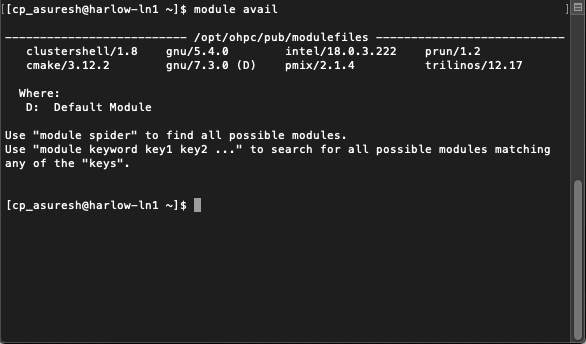
\includegraphics[width=\textwidth]{module_avail.png}
			\caption{Module avail}
		\end{subfigure}
		\begin{subfigure}[h]{0.450\textwidth}
			\centering
			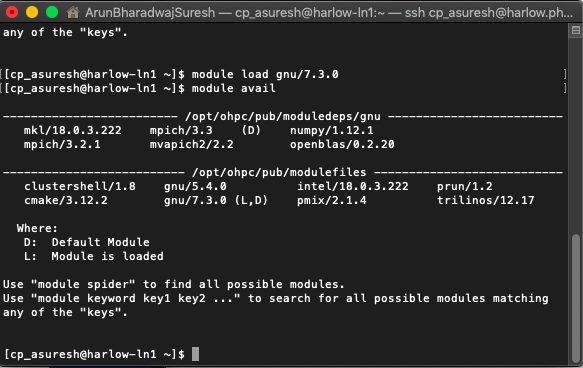
\includegraphics[width=\textwidth]{module_load.png}
			\caption{Module load}
		\end{subfigure}
		\begin{subfigure}[h]{0.450\textwidth}
			\centering
			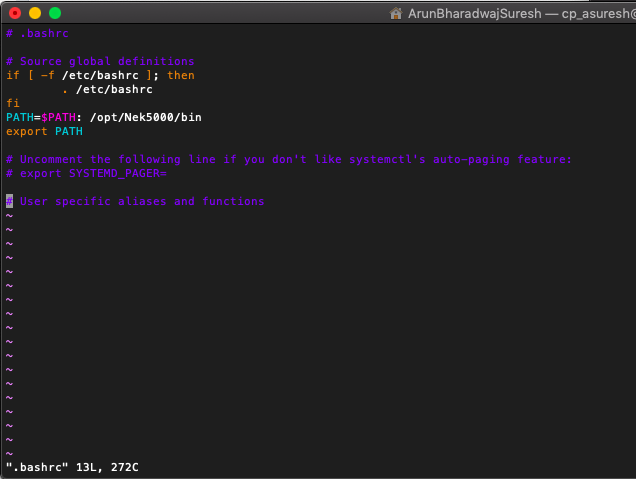
\includegraphics[width=\textwidth]{vim.png}
			\caption{Appended file}
		\end{subfigure}\\ 
\end{figure}
\newpage
\begin{figure}[h]
	\centering
	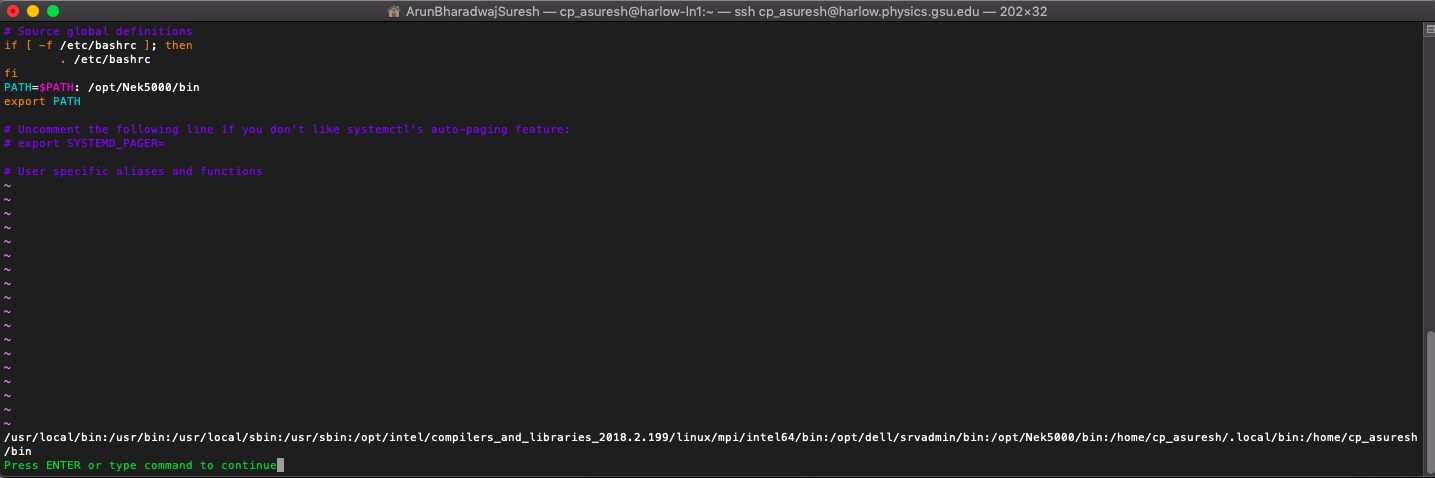
\includegraphics[width=\textwidth]{pathoutput.png}
	\caption{Output}
\end{figure}
\noindent \textbf{Text of the output:}\\ /usr/local/bin:/usr/bin:/usr/local/sbin:/usr/sbin:/opt/intel/compilers\_and\_libraries\_2018.2.199/\\linux/mpi/intel64/bin:/opt/dell/srvadmin/bin\textbf{:/opt/Nek5000/bin}:\\/home/cp\_asuresh/.local/bin:/home/cp\_asuresh
/bin
\end{document}